\documentclass[twoside]{book}

% Packages required by doxygen
\usepackage{fixltx2e}
\usepackage{calc}
\usepackage{doxygen}
\usepackage[export]{adjustbox} % also loads graphicx
\usepackage{graphicx}
\usepackage[utf8]{inputenc}
\usepackage{makeidx}
\usepackage{multicol}
\usepackage{multirow}
\PassOptionsToPackage{warn}{textcomp}
\usepackage{textcomp}
\usepackage[nointegrals]{wasysym}
\usepackage[table]{xcolor}

% Font selection
\usepackage[T1]{fontenc}
\usepackage[scaled=.90]{helvet}
\usepackage{courier}
\usepackage{amssymb}
\usepackage{sectsty}
\renewcommand{\familydefault}{\sfdefault}
\allsectionsfont{%
  \fontseries{bc}\selectfont%
  \color{darkgray}%
}
\renewcommand{\DoxyLabelFont}{%
  \fontseries{bc}\selectfont%
  \color{darkgray}%
}
\newcommand{\+}{\discretionary{\mbox{\scriptsize$\hookleftarrow$}}{}{}}

% Page & text layout
\usepackage{geometry}
\geometry{%
  a4paper,%
  top=2.5cm,%
  bottom=2.5cm,%
  left=2.5cm,%
  right=2.5cm%
}
\tolerance=750
\hfuzz=15pt
\hbadness=750
\setlength{\emergencystretch}{15pt}
\setlength{\parindent}{0cm}
\setlength{\parskip}{3ex plus 2ex minus 2ex}
\makeatletter
\renewcommand{\paragraph}{%
  \@startsection{paragraph}{4}{0ex}{-1.0ex}{1.0ex}{%
    \normalfont\normalsize\bfseries\SS@parafont%
  }%
}
\renewcommand{\subparagraph}{%
  \@startsection{subparagraph}{5}{0ex}{-1.0ex}{1.0ex}{%
    \normalfont\normalsize\bfseries\SS@subparafont%
  }%
}
\makeatother

% Headers & footers
\usepackage{fancyhdr}
\pagestyle{fancyplain}
\fancyhead[LE]{\fancyplain{}{\bfseries\thepage}}
\fancyhead[CE]{\fancyplain{}{}}
\fancyhead[RE]{\fancyplain{}{\bfseries\leftmark}}
\fancyhead[LO]{\fancyplain{}{\bfseries\rightmark}}
\fancyhead[CO]{\fancyplain{}{}}
\fancyhead[RO]{\fancyplain{}{\bfseries\thepage}}
\fancyfoot[LE]{\fancyplain{}{}}
\fancyfoot[CE]{\fancyplain{}{}}
\fancyfoot[RE]{\fancyplain{}{\bfseries\scriptsize Generated by Doxygen }}
\fancyfoot[LO]{\fancyplain{}{\bfseries\scriptsize Generated by Doxygen }}
\fancyfoot[CO]{\fancyplain{}{}}
\fancyfoot[RO]{\fancyplain{}{}}
\renewcommand{\footrulewidth}{0.4pt}
\renewcommand{\chaptermark}[1]{%
  \markboth{#1}{}%
}
\renewcommand{\sectionmark}[1]{%
  \markright{\thesection\ #1}%
}

% Indices & bibliography
\usepackage{natbib}
\usepackage[titles]{tocloft}
\setcounter{tocdepth}{3}
\setcounter{secnumdepth}{5}
\makeindex

% Hyperlinks (required, but should be loaded last)
\usepackage{ifpdf}
\ifpdf
  \usepackage[pdftex,pagebackref=true]{hyperref}
\else
  \usepackage[ps2pdf,pagebackref=true]{hyperref}
\fi
\hypersetup{%
  colorlinks=true,%
  linkcolor=blue,%
  citecolor=blue,%
  unicode%
}

% Custom commands
\newcommand{\clearemptydoublepage}{%
  \newpage{\pagestyle{empty}\cleardoublepage}%
}

\usepackage{caption}
\captionsetup{labelsep=space,justification=centering,font={bf},singlelinecheck=off,skip=4pt,position=top}

%===== C O N T E N T S =====

\begin{document}

% Titlepage & ToC
\hypersetup{pageanchor=false,
             bookmarksnumbered=true,
             pdfencoding=unicode
            }
\pagenumbering{alph}
\begin{titlepage}
\vspace*{7cm}
\begin{center}%
{\Large Side\+Fog\+Cube \\[1ex]\large 1.\+0 }\\
\vspace*{1cm}
{\large Generated by Doxygen 1.8.13}\\
\end{center}
\end{titlepage}
\clearemptydoublepage
\pagenumbering{roman}
\tableofcontents
\clearemptydoublepage
\pagenumbering{arabic}
\hypersetup{pageanchor=true}

%--- Begin generated contents ---
\chapter{Hierarchical Index}
\section{Class Hierarchy}
This inheritance list is sorted roughly, but not completely, alphabetically\+:\begin{DoxyCompactList}
\item \contentsline{section}{Camera}{\pageref{classCamera}}{}
\item C\+L\+\_\+\+Clan\+Application\begin{DoxyCompactList}
\item \contentsline{section}{Side\+Fog\+Cube}{\pageref{classSideFogCube}}{}
\end{DoxyCompactList}
\item \contentsline{section}{Common\+Header}{\pageref{classCommonHeader}}{}
\item \contentsline{section}{Create\+Image}{\pageref{classCreateImage}}{}
\item \contentsline{section}{Inst\+Data}{\pageref{structInstData}}{}
\item \contentsline{section}{Lights}{\pageref{structLights}}{}
\item \contentsline{section}{Pos\+Orient}{\pageref{structPosOrient}}{}
\item \contentsline{section}{Shader}{\pageref{classShader}}{}
\item \contentsline{section}{Uniform\+Printer}{\pageref{classUniformPrinter}}{}
\end{DoxyCompactList}

\chapter{Class Index}
\section{Class List}
Here are the classes, structs, unions and interfaces with brief descriptions\+:\begin{DoxyCompactList}
\item\contentsline{section}{\hyperlink{classCamera}{Camera} }{\pageref{classCamera}}{}
\item\contentsline{section}{\hyperlink{classCommonHeader}{Common\+Header} }{\pageref{classCommonHeader}}{}
\item\contentsline{section}{\hyperlink{classCreateImage}{Create\+Image} }{\pageref{classCreateImage}}{}
\item\contentsline{section}{\hyperlink{structInstData}{Inst\+Data} \\*Data for the buffer going to the shader }{\pageref{structInstData}}{}
\item\contentsline{section}{\hyperlink{structLights}{Lights} \\*Structure for the uniform holding the lighting data }{\pageref{structLights}}{}
\item\contentsline{section}{\hyperlink{structPosOrient}{Pos\+Orient} }{\pageref{structPosOrient}}{}
\item\contentsline{section}{\hyperlink{classShader}{Shader} }{\pageref{classShader}}{}
\item\contentsline{section}{\hyperlink{classSideFogCube}{Side\+Fog\+Cube} }{\pageref{classSideFogCube}}{}
\item\contentsline{section}{\hyperlink{classUniformPrinter}{Uniform\+Printer} }{\pageref{classUniformPrinter}}{}
\end{DoxyCompactList}

\chapter{Class Documentation}
\hypertarget{classCamera}{}\section{Camera Class Reference}
\label{classCamera}\index{Camera@{Camera}}


{\ttfamily \#include $<$camera.\+h$>$}

\subsection*{Public Types}
\begin{DoxyCompactItemize}
\item 
\mbox{\Hypertarget{classCamera_a910e91793a0078a11eef1cba77dec353}\label{classCamera_a910e91793a0078a11eef1cba77dec353}} 
enum \hyperlink{classCamera_a910e91793a0078a11eef1cba77dec353}{Camera\+\_\+\+Movement} \{ \newline
{\bfseries F\+O\+R\+W\+A\+RD}, 
{\bfseries B\+A\+C\+K\+W\+A\+RD}, 
{\bfseries L\+E\+FT}, 
{\bfseries R\+I\+G\+HT}, 
\newline
{\bfseries C\+L\+O\+S\+ER}, 
{\bfseries A\+W\+AY}, 
{\bfseries UP}, 
{\bfseries D\+O\+WN}
 \}\begin{DoxyCompactList}\small\item\em \hyperlink{classCamera}{Camera} Movement Defines several possible options for camera movement. Used as an abstraction to stay away from window-\/system specific input methods. To access this from the calling class use \char`\"{}\+Camera\+::\+Camera\+\_\+\+Movement\+::\+F\+O\+R\+W\+A\+R\+D\char`\"{}, etc. \end{DoxyCompactList}
\end{DoxyCompactItemize}
\subsection*{Public Member Functions}
\begin{DoxyCompactItemize}
\item 
\hyperlink{classCamera_ab7a973c909384f298849f8b8cc78f96a}{Camera} (int width, int height, vec3 \hyperlink{classCamera_a6bd96884fb5fb652b71042f2d7f0122c}{position}=vec3(0.\+0f, 0.\+0f, 0.\+0f), vec3 up=vec3(0.\+0f, 1.\+0f, 0.\+0f), float yaw=\+Y\+A\+W, float pitch=\+P\+I\+T\+C\+H)
\begin{DoxyCompactList}\small\item\em \hyperlink{classCamera}{Camera} Constructor with vectors. \end{DoxyCompactList}\item 
\mbox{\Hypertarget{classCamera_a63f2b4fd5bbd47ed7634116425d63d94}\label{classCamera_a63f2b4fd5bbd47ed7634116425d63d94}} 
\hyperlink{classCamera_a63f2b4fd5bbd47ed7634116425d63d94}{Camera} (int width, int height, float posX, float posY, float posZ, float upX, float upY, float upZ, float yaw, float pitch)
\begin{DoxyCompactList}\small\item\em \hyperlink{classCamera}{Camera} Constructor with variables. \end{DoxyCompactList}\item 
\mbox{\Hypertarget{classCamera_aff6521263c6ecba92fa98a8e9e4461bf}\label{classCamera_aff6521263c6ecba92fa98a8e9e4461bf}} 
mat4 \hyperlink{classCamera_aff6521263c6ecba92fa98a8e9e4461bf}{Get\+View\+Matrix} ()
\begin{DoxyCompactList}\small\item\em Get\+View\+Matrix Returns the view matrix calculated using Euler Angles and the Look\+At matrix. \end{DoxyCompactList}\item 
\mbox{\Hypertarget{classCamera_a9c08d56907d6122c9214f30194657252}\label{classCamera_a9c08d56907d6122c9214f30194657252}} 
mat4 \hyperlink{classCamera_a9c08d56907d6122c9214f30194657252}{Get\+Perspective} ()
\begin{DoxyCompactList}\small\item\em Get\+Perspective Returns the look\+At matrix. \end{DoxyCompactList}\item 
\mbox{\Hypertarget{classCamera_aee8027b5309a5dc77db956d27924c387}\label{classCamera_aee8027b5309a5dc77db956d27924c387}} 
void \hyperlink{classCamera_aee8027b5309a5dc77db956d27924c387}{reset\+Camera} ()
\begin{DoxyCompactList}\small\item\em reset\+Camera Resets the camera to the original position and zoom. \end{DoxyCompactList}\item 
\mbox{\Hypertarget{classCamera_aa645c28c6739e6ede0a238e8b3587d69}\label{classCamera_aa645c28c6739e6ede0a238e8b3587d69}} 
vec3 \hyperlink{classCamera_aa645c28c6739e6ede0a238e8b3587d69}{Get\+Position} ()
\begin{DoxyCompactList}\small\item\em Get\+Position Returns the camera position. \end{DoxyCompactList}\item 
\mbox{\Hypertarget{classCamera_ab31c607f43c69ca3b625589675a225c6}\label{classCamera_ab31c607f43c69ca3b625589675a225c6}} 
void \hyperlink{classCamera_ab31c607f43c69ca3b625589675a225c6}{Set\+Position} (vec3 \hyperlink{classCamera_a6bd96884fb5fb652b71042f2d7f0122c}{position})
\begin{DoxyCompactList}\small\item\em Set\+Position Sets the camera position. \end{DoxyCompactList}\item 
void \hyperlink{classCamera_aebba33a8b281fe2598bcafc54a55d296}{Process\+Keyboard} (\hyperlink{classCamera_a910e91793a0078a11eef1cba77dec353}{Camera\+\_\+\+Movement} direction, float delta\+Time)
\begin{DoxyCompactList}\small\item\em Process\+Keyboard Processes input received from any keyboard-\/like input system. Accepts input parameter in the form of camera defined E\+N\+UM (to abstract it from windowing systems) \end{DoxyCompactList}\item 
void \hyperlink{classCamera_a656c2a8dc40150874f15bce47b789751}{Process\+Mouse\+Movement} (float xoffset, float yoffset, G\+Lboolean constrain\+Pitch=true)
\begin{DoxyCompactList}\small\item\em Process\+Mouse\+Movement Processes input received from a mouse input system. Expects the offset value in both the x and y direction. \end{DoxyCompactList}\item 
void \hyperlink{classCamera_a17373e11b6b64a0568ce2a03b48ec067}{Process\+Mouse\+Scroll} (\hyperlink{classCamera_a910e91793a0078a11eef1cba77dec353}{Camera\+\_\+\+Movement} inout)
\begin{DoxyCompactList}\small\item\em Process\+Mouse\+Scroll Processes input received from a mouse scroll-\/wheel event. Only requires input on the vertical wheel-\/axis. \end{DoxyCompactList}\end{DoxyCompactItemize}
\subsection*{Public Attributes}
\begin{DoxyCompactItemize}
\item 
\mbox{\Hypertarget{classCamera_a28ae256428afe91a894b99584bdcfe4f}\label{classCamera_a28ae256428afe91a894b99584bdcfe4f}} 
vec3 \hyperlink{classCamera_a28ae256428afe91a894b99584bdcfe4f}{Position}
\begin{DoxyCompactList}\small\item\em \hyperlink{classCamera}{Camera} Attributes. \end{DoxyCompactList}\item 
\mbox{\Hypertarget{classCamera_ae8fefdb9e27290a00d9c70be77086bc6}\label{classCamera_ae8fefdb9e27290a00d9c70be77086bc6}} 
vec3 {\bfseries Front}
\item 
\mbox{\Hypertarget{classCamera_a17c45b2bf09c165a4cf1aff793f628d7}\label{classCamera_a17c45b2bf09c165a4cf1aff793f628d7}} 
vec3 {\bfseries Up}
\item 
\mbox{\Hypertarget{classCamera_a1c47a3264f5bc15356de0319df40696a}\label{classCamera_a1c47a3264f5bc15356de0319df40696a}} 
vec3 {\bfseries Right}
\item 
\mbox{\Hypertarget{classCamera_a45f586b01107a672129db3381e60e3f0}\label{classCamera_a45f586b01107a672129db3381e60e3f0}} 
vec3 {\bfseries World\+Up}
\item 
vec3 \hyperlink{classCamera_a6bd96884fb5fb652b71042f2d7f0122c}{position}
\item 
\mbox{\Hypertarget{classCamera_a21683f89507e000b6a0ebabff08ac8a2}\label{classCamera_a21683f89507e000b6a0ebabff08ac8a2}} 
vec3 {\bfseries up\+Orig}
\item 
\mbox{\Hypertarget{classCamera_a1a1354a2bd2df7f18ef82924e671d241}\label{classCamera_a1a1354a2bd2df7f18ef82924e671d241}} 
float \hyperlink{classCamera_a1a1354a2bd2df7f18ef82924e671d241}{Yaw}
\begin{DoxyCompactList}\small\item\em Euler Angles. \end{DoxyCompactList}\item 
\mbox{\Hypertarget{classCamera_af9c8f223bb06bb74fc77c586545e7e67}\label{classCamera_af9c8f223bb06bb74fc77c586545e7e67}} 
float {\bfseries Pitch}
\item 
\mbox{\Hypertarget{classCamera_a63221392d762df6a74f45bc9d43a2f61}\label{classCamera_a63221392d762df6a74f45bc9d43a2f61}} 
float {\bfseries Movement\+Speed}
\item 
\mbox{\Hypertarget{classCamera_a73e88844b31d5111eeb76327dfbb2d68}\label{classCamera_a73e88844b31d5111eeb76327dfbb2d68}} 
float {\bfseries Mouse\+Sensitivity}
\item 
\mbox{\Hypertarget{classCamera_a2becf27d08eb7e6da9c597c73ea95b5d}\label{classCamera_a2becf27d08eb7e6da9c597c73ea95b5d}} 
float {\bfseries Zoom}
\item 
\mbox{\Hypertarget{classCamera_a7f3890bf4c4bd76790569c1c42014e32}\label{classCamera_a7f3890bf4c4bd76790569c1c42014e32}} 
int {\bfseries width}
\item 
\mbox{\Hypertarget{classCamera_a71d4b6a3a1bcd937a9f147a3e35a8fed}\label{classCamera_a71d4b6a3a1bcd937a9f147a3e35a8fed}} 
int {\bfseries height}
\item 
\mbox{\Hypertarget{classCamera_a94693ab302c858a511a44a4f34ef64ae}\label{classCamera_a94693ab302c858a511a44a4f34ef64ae}} 
mat4 {\bfseries projection}
\end{DoxyCompactItemize}
\subsection*{Static Public Attributes}
\begin{DoxyCompactItemize}
\item 
\mbox{\Hypertarget{classCamera_a409bc996200b4781bb35cff69bc700ae}\label{classCamera_a409bc996200b4781bb35cff69bc700ae}} 
static constexpr float \hyperlink{classCamera_a409bc996200b4781bb35cff69bc700ae}{Y\+AW} = -\/90.\+0f
\begin{DoxyCompactList}\small\item\em Default camera values. \end{DoxyCompactList}\item 
\mbox{\Hypertarget{classCamera_a1a3c7b1d1fe585faf2224ccd6c2614e3}\label{classCamera_a1a3c7b1d1fe585faf2224ccd6c2614e3}} 
static constexpr float {\bfseries P\+I\+T\+CH} = 0.\+0f
\item 
\mbox{\Hypertarget{classCamera_af80c8fa98a4f3261080ed80527ba7f80}\label{classCamera_af80c8fa98a4f3261080ed80527ba7f80}} 
static constexpr float {\bfseries S\+P\+E\+ED} = 0.\+5f
\item 
\mbox{\Hypertarget{classCamera_a06474967f88b6cd3023a5c6fe4c49601}\label{classCamera_a06474967f88b6cd3023a5c6fe4c49601}} 
static constexpr float {\bfseries S\+E\+N\+S\+I\+T\+I\+V\+I\+TY} = 0.\+3f
\item 
\mbox{\Hypertarget{classCamera_a27bbb30d1b08f4e2d3c4342b60487301}\label{classCamera_a27bbb30d1b08f4e2d3c4342b60487301}} 
static constexpr float {\bfseries Z\+O\+OM} = 45.\+0f
\item 
\mbox{\Hypertarget{classCamera_a2020859c32befc6e4261240b15ff7b33}\label{classCamera_a2020859c32befc6e4261240b15ff7b33}} 
static constexpr float {\bfseries onedegree} = (float) acos(-\/1) / 180.\+0f
\end{DoxyCompactItemize}


\subsection{Detailed Description}
An abstract camera class that processes input and calculates the corresponding Euler Angles, Vectors and Matrices for moving the camera about a 3-\/dimensional landscape. For use in Open\+GL. 

Definition at line 19 of file camera.\+h.



\subsection{Constructor \& Destructor Documentation}
\mbox{\Hypertarget{classCamera_ab7a973c909384f298849f8b8cc78f96a}\label{classCamera_ab7a973c909384f298849f8b8cc78f96a}} 
\index{Camera@{Camera}!Camera@{Camera}}
\index{Camera@{Camera}!Camera@{Camera}}
\subsubsection{\texorpdfstring{Camera()}{Camera()}}
{\footnotesize\ttfamily Camera\+::\+Camera (\begin{DoxyParamCaption}\item[{int}]{width,  }\item[{int}]{height,  }\item[{vec3}]{position = {\ttfamily vec3(0.0f,~0.0f,~0.0f)},  }\item[{vec3}]{up = {\ttfamily vec3(0.0f,~1.0f,~0.0f)},  }\item[{float}]{yaw = {\ttfamily \hyperlink{classCamera_a409bc996200b4781bb35cff69bc700ae}{Y\+AW}},  }\item[{float}]{pitch = {\ttfamily PITCH} }\end{DoxyParamCaption})}



\hyperlink{classCamera}{Camera} Constructor with vectors. 

Constructor with vectors. 

Definition at line 11 of file camera.\+cpp.



\subsection{Member Function Documentation}
\mbox{\Hypertarget{classCamera_aebba33a8b281fe2598bcafc54a55d296}\label{classCamera_aebba33a8b281fe2598bcafc54a55d296}} 
\index{Camera@{Camera}!Process\+Keyboard@{Process\+Keyboard}}
\index{Process\+Keyboard@{Process\+Keyboard}!Camera@{Camera}}
\subsubsection{\texorpdfstring{Process\+Keyboard()}{ProcessKeyboard()}}
{\footnotesize\ttfamily void Camera\+::\+Process\+Keyboard (\begin{DoxyParamCaption}\item[{\hyperlink{classCamera_a910e91793a0078a11eef1cba77dec353}{Camera\+\_\+\+Movement}}]{direction,  }\item[{float}]{delta\+Time }\end{DoxyParamCaption})}



Process\+Keyboard Processes input received from any keyboard-\/like input system. Accepts input parameter in the form of camera defined E\+N\+UM (to abstract it from windowing systems) 

Move the camera around the scene. 

Definition at line 72 of file camera.\+cpp.

\mbox{\Hypertarget{classCamera_a656c2a8dc40150874f15bce47b789751}\label{classCamera_a656c2a8dc40150874f15bce47b789751}} 
\index{Camera@{Camera}!Process\+Mouse\+Movement@{Process\+Mouse\+Movement}}
\index{Process\+Mouse\+Movement@{Process\+Mouse\+Movement}!Camera@{Camera}}
\subsubsection{\texorpdfstring{Process\+Mouse\+Movement()}{ProcessMouseMovement()}}
{\footnotesize\ttfamily void Camera\+::\+Process\+Mouse\+Movement (\begin{DoxyParamCaption}\item[{float}]{xoffset,  }\item[{float}]{yoffset,  }\item[{G\+Lboolean}]{constrain\+Pitch = {\ttfamily true} }\end{DoxyParamCaption})}



Process\+Mouse\+Movement Processes input received from a mouse input system. Expects the offset value in both the x and y direction. 

Point the camera according to the mouse motion.

Make sure that when pitch is out of bounds, screen doesn\textquotesingle{}t get flipped

Update Front, Right and Up Vectors using the updated Euler angles 

Definition at line 91 of file camera.\+cpp.

\mbox{\Hypertarget{classCamera_a17373e11b6b64a0568ce2a03b48ec067}\label{classCamera_a17373e11b6b64a0568ce2a03b48ec067}} 
\index{Camera@{Camera}!Process\+Mouse\+Scroll@{Process\+Mouse\+Scroll}}
\index{Process\+Mouse\+Scroll@{Process\+Mouse\+Scroll}!Camera@{Camera}}
\subsubsection{\texorpdfstring{Process\+Mouse\+Scroll()}{ProcessMouseScroll()}}
{\footnotesize\ttfamily void Camera\+::\+Process\+Mouse\+Scroll (\begin{DoxyParamCaption}\item[{\hyperlink{classCamera_a910e91793a0078a11eef1cba77dec353}{Camera\+\_\+\+Movement}}]{inout }\end{DoxyParamCaption})}



Process\+Mouse\+Scroll Processes input received from a mouse scroll-\/wheel event. Only requires input on the vertical wheel-\/axis. 

Handles zoom in and zoom out. 

Definition at line 113 of file camera.\+cpp.



\subsection{Member Data Documentation}
\mbox{\Hypertarget{classCamera_a6bd96884fb5fb652b71042f2d7f0122c}\label{classCamera_a6bd96884fb5fb652b71042f2d7f0122c}} 
\index{Camera@{Camera}!position@{position}}
\index{position@{position}!Camera@{Camera}}
\subsubsection{\texorpdfstring{position}{position}}
{\footnotesize\ttfamily vec3 Camera\+::position}

Theses two variables are to capture data for the reset\+Camera function. 

Definition at line 55 of file camera.\+h.



The documentation for this class was generated from the following files\+:\begin{DoxyCompactItemize}
\item 
camera.\+h\item 
camera.\+cpp\end{DoxyCompactItemize}

\hypertarget{classCommonHeader}{}\section{Common\+Header Class Reference}
\label{classCommonHeader}\index{Common\+Header@{Common\+Header}}


{\ttfamily \#include $<$commonheader.\+h$>$}



\subsection{Detailed Description}
A header file to reduce repetition of \#define and \#include statements. 

The documentation for this class was generated from the following file\+:\begin{DoxyCompactItemize}
\item 
commonheader.\+h\end{DoxyCompactItemize}

\hypertarget{classCreateImage}{}\section{Create\+Image Class Reference}
\label{classCreateImage}\index{Create\+Image@{Create\+Image}}
\subsection*{Public Member Functions}
\begin{DoxyCompactItemize}
\item 
void \hyperlink{classCreateImage_a0fb8715c56dc5ff120aa355ca66496f6}{set\+Image} (string imagefile)
\begin{DoxyCompactList}\small\item\em set\+Image Load image and convert it. \end{DoxyCompactList}\item 
G\+Lsizei \hyperlink{classCreateImage_ac0edbffce968346bd4c43564beb27c26}{get\+Width} ()
\begin{DoxyCompactList}\small\item\em get\+Width Accessor function. \end{DoxyCompactList}\item 
\mbox{\Hypertarget{classCreateImage_abeb628a5f2fc67aeb1c39c1d0a445142}\label{classCreateImage_abeb628a5f2fc67aeb1c39c1d0a445142}} 
G\+Lsizei \hyperlink{classCreateImage_abeb628a5f2fc67aeb1c39c1d0a445142}{get\+Height} ()
\begin{DoxyCompactList}\small\item\em get\+Height Accessor function. \end{DoxyCompactList}\item 
\mbox{\Hypertarget{classCreateImage_a85dfaf7a1b8bf86c12877b117f8989b8}\label{classCreateImage_a85dfaf7a1b8bf86c12877b117f8989b8}} 
G\+Lvoid $\ast$ \hyperlink{classCreateImage_a85dfaf7a1b8bf86c12877b117f8989b8}{get\+Data} ()
\begin{DoxyCompactList}\small\item\em get\+Data Accessor function. \end{DoxyCompactList}\item 
G\+Luint \hyperlink{classCreateImage_a529a1307050df8719e180e006141b762}{texture\+Object} ()
\begin{DoxyCompactList}\small\item\em texture\+Object Return an Open\+GL buffer object. \end{DoxyCompactList}\item 
void \hyperlink{classCreateImage_acbff5ee9dfb7e64bcf850cce6f3ee13d}{create\+Sky\+Box\+Tex} (G\+Luint \&texture\+ID, string filenames\mbox{[}6\mbox{]})
\begin{DoxyCompactList}\small\item\em create\+Sky\+Box\+Tex Create a sky box using six pictures for the inside of the box. \end{DoxyCompactList}\item 
void \hyperlink{classCreateImage_a51bb6307d7b106aab55292813ef8b694}{create2\+D\+Tex\+Array} (G\+Luint \&texture\+ID, string filenames\mbox{[}16\mbox{]})
\begin{DoxyCompactList}\small\item\em create2\+D\+Tex\+Array Create a texture array, you can adjust this to make up to a maximum picture array size of 256. \end{DoxyCompactList}\end{DoxyCompactItemize}
\subsection*{Protected Attributes}
\begin{DoxyCompactItemize}
\item 
\mbox{\Hypertarget{classCreateImage_aef75789ae909e699137dd13bfb6c8ae3}\label{classCreateImage_aef75789ae909e699137dd13bfb6c8ae3}} 
fip\+Image \hyperlink{classCreateImage_aef75789ae909e699137dd13bfb6c8ae3}{txt\+Image}
\begin{DoxyCompactList}\small\item\em Class global variables. \end{DoxyCompactList}\item 
\mbox{\Hypertarget{classCreateImage_a75be3bf73393293b28bf3a4f67c2acfb}\label{classCreateImage_a75be3bf73393293b28bf3a4f67c2acfb}} 
B\+Y\+TE $\ast$ {\bfseries pic\+Line}
\item 
\mbox{\Hypertarget{classCreateImage_a820c4459b175116be89caf19a46926ae}\label{classCreateImage_a820c4459b175116be89caf19a46926ae}} 
G\+Lsizei {\bfseries width}
\item 
\mbox{\Hypertarget{classCreateImage_a2932fbd279fc1407a74fbfa37d2857df}\label{classCreateImage_a2932fbd279fc1407a74fbfa37d2857df}} 
G\+Lsizei {\bfseries height}
\item 
\mbox{\Hypertarget{classCreateImage_a409d26c7a384b82b0638c25a2b6b2194}\label{classCreateImage_a409d26c7a384b82b0638c25a2b6b2194}} 
int {\bfseries size} = 0
\item 
\mbox{\Hypertarget{classCreateImage_a8ac66363719dbbba5386527ec970c2fe}\label{classCreateImage_a8ac66363719dbbba5386527ec970c2fe}} 
unsigned char $\ast$ {\bfseries pixels} = N\+U\+LL
\item 
\mbox{\Hypertarget{classCreateImage_a52d1bf19d5ca8be287e93b811fc29d2f}\label{classCreateImage_a52d1bf19d5ca8be287e93b811fc29d2f}} 
int {\bfseries count}
\item 
\mbox{\Hypertarget{classCreateImage_aaeeb240ef49097e5968c02996dcd7b01}\label{classCreateImage_aaeeb240ef49097e5968c02996dcd7b01}} 
int {\bfseries line}
\end{DoxyCompactItemize}


\subsection{Detailed Description}


Definition at line 29 of file createimage.\+h.



\subsection{Member Function Documentation}
\mbox{\Hypertarget{classCreateImage_a51bb6307d7b106aab55292813ef8b694}\label{classCreateImage_a51bb6307d7b106aab55292813ef8b694}} 
\index{Create\+Image@{Create\+Image}!create2\+D\+Tex\+Array@{create2\+D\+Tex\+Array}}
\index{create2\+D\+Tex\+Array@{create2\+D\+Tex\+Array}!Create\+Image@{Create\+Image}}
\subsubsection{\texorpdfstring{create2\+D\+Tex\+Array()}{create2DTexArray()}}
{\footnotesize\ttfamily void Create\+Image\+::create2\+D\+Tex\+Array (\begin{DoxyParamCaption}\item[{G\+Luint \&}]{texture\+ID,  }\item[{string}]{filenames\mbox{[}16\mbox{]} }\end{DoxyParamCaption})}



create2\+D\+Tex\+Array Create a texture array, you can adjust this to make up to a maximum picture array size of 256. 

Loads a texture array that can be up to 256 pictures in size. The pictures should be of the same type. and the same dimensions (pixel width and pixel height). They are loaded one after another into the buffer which is then loaded into the shader. The system accounts for each picture by knowing the size of a picture in the array.

The variable size below is determined by the background crate image which is of the same size and type as the pictures used in the array.

! Six images, one texture ID.

width = \hyperlink{classCreateImage_ac0edbffce968346bd4c43564beb27c26}{get\+Width()}; height = \hyperlink{classCreateImage_abeb628a5f2fc67aeb1c39c1d0a445142}{get\+Height()}; 

Definition at line 159 of file createimage.\+cpp.

\mbox{\Hypertarget{classCreateImage_acbff5ee9dfb7e64bcf850cce6f3ee13d}\label{classCreateImage_acbff5ee9dfb7e64bcf850cce6f3ee13d}} 
\index{Create\+Image@{Create\+Image}!create\+Sky\+Box\+Tex@{create\+Sky\+Box\+Tex}}
\index{create\+Sky\+Box\+Tex@{create\+Sky\+Box\+Tex}!Create\+Image@{Create\+Image}}
\subsubsection{\texorpdfstring{create\+Sky\+Box\+Tex()}{createSkyBoxTex()}}
{\footnotesize\ttfamily void Create\+Image\+::create\+Sky\+Box\+Tex (\begin{DoxyParamCaption}\item[{G\+Luint \&}]{texture\+ID,  }\item[{string}]{filenames\mbox{[}6\mbox{]} }\end{DoxyParamCaption})}



create\+Sky\+Box\+Tex Create a sky box using six pictures for the inside of the box. 

Loads a cubemap texture from 6 individual texture faces Order should be\+: +X (right) -\/X (left) +Y (top) -\/Y (bottom) +Z (front) -\/Z (back)

Six images, one texture ID. 

Definition at line 126 of file createimage.\+cpp.

\mbox{\Hypertarget{classCreateImage_ac0edbffce968346bd4c43564beb27c26}\label{classCreateImage_ac0edbffce968346bd4c43564beb27c26}} 
\index{Create\+Image@{Create\+Image}!get\+Width@{get\+Width}}
\index{get\+Width@{get\+Width}!Create\+Image@{Create\+Image}}
\subsubsection{\texorpdfstring{get\+Width()}{getWidth()}}
{\footnotesize\ttfamily G\+Lsizei Create\+Image\+::get\+Width (\begin{DoxyParamCaption}{ }\end{DoxyParamCaption})}



get\+Width Accessor function. 

! Accessor functions to pass along the data. 

Definition at line 89 of file createimage.\+cpp.

\mbox{\Hypertarget{classCreateImage_a0fb8715c56dc5ff120aa355ca66496f6}\label{classCreateImage_a0fb8715c56dc5ff120aa355ca66496f6}} 
\index{Create\+Image@{Create\+Image}!set\+Image@{set\+Image}}
\index{set\+Image@{set\+Image}!Create\+Image@{Create\+Image}}
\subsubsection{\texorpdfstring{set\+Image()}{setImage()}}
{\footnotesize\ttfamily void Create\+Image\+::set\+Image (\begin{DoxyParamCaption}\item[{string}]{imagefile }\end{DoxyParamCaption})}



set\+Image Load image and convert it. 

all the image files are required to be in an images directory.

! Delete the item if it exists.

! Free Image Plus Image loads any standard picture.

! Convert image to four 8 bit fields R\+G\+BA.

Load the image into an unsigned char array. 

Definition at line 23 of file createimage.\+cpp.

\mbox{\Hypertarget{classCreateImage_a529a1307050df8719e180e006141b762}\label{classCreateImage_a529a1307050df8719e180e006141b762}} 
\index{Create\+Image@{Create\+Image}!texture\+Object@{texture\+Object}}
\index{texture\+Object@{texture\+Object}!Create\+Image@{Create\+Image}}
\subsubsection{\texorpdfstring{texture\+Object()}{textureObject()}}
{\footnotesize\ttfamily G\+Luint Create\+Image\+::texture\+Object (\begin{DoxyParamCaption}{ }\end{DoxyParamCaption})}



texture\+Object Return an Open\+GL buffer object. 

! Use the \hyperlink{classCreateImage}{Create\+Image} class to turn an image into a texture. Generate texture ID and load texture data

Parameters 

Definition at line 105 of file createimage.\+cpp.



The documentation for this class was generated from the following files\+:\begin{DoxyCompactItemize}
\item 
createimage.\+h\item 
createimage.\+cpp\end{DoxyCompactItemize}

\hypertarget{structInstData}{}\section{Inst\+Data Struct Reference}
\label{structInstData}\index{Inst\+Data@{Inst\+Data}}


Data for the buffer going to the shader.  




{\ttfamily \#include $<$commonheader.\+h$>$}

\subsection*{Public Attributes}
\begin{DoxyCompactItemize}
\item 
\mbox{\Hypertarget{structInstData_ae3c2b0364b5744758cf1759228dcf21d}\label{structInstData_ae3c2b0364b5744758cf1759228dcf21d}} 
vec4 {\bfseries inst\+Index1} \mbox{[}N\+U\+M\+\_\+\+I\+M\+A\+G\+ES $\ast$N\+U\+M\+\_\+\+I\+N\+S\+T\+A\+N\+C\+ES\mbox{]}
\item 
\mbox{\Hypertarget{structInstData_aaf5f6b2d5a390f70d422a2a0a18ab809}\label{structInstData_aaf5f6b2d5a390f70d422a2a0a18ab809}} 
vec2 {\bfseries inst\+Index2} \mbox{[}N\+U\+M\+\_\+\+I\+M\+A\+G\+ES $\ast$N\+U\+M\+\_\+\+I\+N\+S\+T\+A\+N\+C\+ES\mbox{]}
\item 
\mbox{\Hypertarget{structInstData_a2c24d884e11884a0156a7f5b3cc674ca}\label{structInstData_a2c24d884e11884a0156a7f5b3cc674ca}} 
vec2 {\bfseries distance} \mbox{[}N\+U\+M\+\_\+\+I\+M\+A\+G\+ES $\ast$N\+U\+M\+\_\+\+I\+N\+S\+T\+A\+N\+C\+ES\mbox{]}
\item 
\mbox{\Hypertarget{structInstData_a5ca34ab9e0b0a80af5f28b3a2d4e6c23}\label{structInstData_a5ca34ab9e0b0a80af5f28b3a2d4e6c23}} 
mat4 {\bfseries inst\+Model} \mbox{[}N\+U\+M\+\_\+\+I\+M\+A\+G\+ES $\ast$N\+U\+M\+\_\+\+I\+N\+S\+T\+A\+N\+C\+ES\mbox{]}
\end{DoxyCompactItemize}


\subsection{Detailed Description}
Data for the buffer going to the shader. 

Definition at line 80 of file commonheader.\+h.



The documentation for this struct was generated from the following file\+:\begin{DoxyCompactItemize}
\item 
commonheader.\+h\end{DoxyCompactItemize}

\hypertarget{structLights}{}\section{Lights Struct Reference}
\label{structLights}\index{Lights@{Lights}}


Structure for the uniform holding the lighting data.  




{\ttfamily \#include $<$commonheader.\+h$>$}

\subsection*{Public Attributes}
\begin{DoxyCompactItemize}
\item 
\mbox{\Hypertarget{structLights_a346d1c9e1feac0aa14dc21719238e0ea}\label{structLights_a346d1c9e1feac0aa14dc21719238e0ea}} 
vec3 {\bfseries light\+Pos}
\item 
\mbox{\Hypertarget{structLights_ae03bc1a0f94b14b6239ba3a0494b081c}\label{structLights_ae03bc1a0f94b14b6239ba3a0494b081c}} 
vec4 {\bfseries light\+Color}
\end{DoxyCompactItemize}


\subsection{Detailed Description}
Structure for the uniform holding the lighting data. 

Definition at line 88 of file commonheader.\+h.



The documentation for this struct was generated from the following file\+:\begin{DoxyCompactItemize}
\item 
commonheader.\+h\end{DoxyCompactItemize}

\hypertarget{structPosOrient}{}\section{Pos\+Orient Struct Reference}
\label{structPosOrient}\index{Pos\+Orient@{Pos\+Orient}}


{\ttfamily \#include $<$commonheader.\+h$>$}

\subsection*{Public Attributes}
\begin{DoxyCompactItemize}
\item 
\mbox{\Hypertarget{structPosOrient_ada336cf840d1815329950b7382b8bb26}\label{structPosOrient_ada336cf840d1815329950b7382b8bb26}} 
vec3 {\bfseries locon}
\item 
\mbox{\Hypertarget{structPosOrient_a83982e054e182fe9f3788efe13b60e94}\label{structPosOrient_a83982e054e182fe9f3788efe13b60e94}} 
double {\bfseries dist}
\item 
\mbox{\Hypertarget{structPosOrient_a416da340d93a46c0f636baccf6983611}\label{structPosOrient_a416da340d93a46c0f636baccf6983611}} 
float {\bfseries index} \mbox{[}6\mbox{]}
\item 
\mbox{\Hypertarget{structPosOrient_a6f5f29c42db9bf7ab943bf0a251d239c}\label{structPosOrient_a6f5f29c42db9bf7ab943bf0a251d239c}} 
float {\bfseries angles}
\item 
\mbox{\Hypertarget{structPosOrient_ae10c9eb375892ee86589bd0409037356}\label{structPosOrient_ae10c9eb375892ee86589bd0409037356}} 
vec3 {\bfseries xaxis}
\item 
\mbox{\Hypertarget{structPosOrient_aa2ff77e127820352715dfd9969d9e0c2}\label{structPosOrient_aa2ff77e127820352715dfd9969d9e0c2}} 
vec3 {\bfseries yaxis}
\end{DoxyCompactItemize}


\subsection{Detailed Description}
Structures to manage the location and data associated with each object. 

Definition at line 70 of file commonheader.\+h.



The documentation for this struct was generated from the following file\+:\begin{DoxyCompactItemize}
\item 
commonheader.\+h\end{DoxyCompactItemize}

\hypertarget{classShader}{}\section{Shader Class Reference}
\label{classShader}\index{Shader@{Shader}}


{\ttfamily \#include $<$shader.\+h$>$}

\subsection*{Public Member Functions}
\begin{DoxyCompactItemize}
\item 
void \hyperlink{classShader_af73d7e0d84dcdcfe0beb871ac796928c}{init\+Shader} (string vertex\+Path, string fragment\+Path, string output\+File)
\begin{DoxyCompactList}\small\item\em init\+Shader Read and build the shader from two files. \end{DoxyCompactList}\item 
unsigned int \hyperlink{classShader_a5a9535209cf2d04bbeff96f8a945f227}{create\+Shader} (unsigned int type, string fpath)
\begin{DoxyCompactList}\small\item\em create\+Shader Create the vertex or fragment shader from a file. \end{DoxyCompactList}\item 
\mbox{\Hypertarget{classShader_a6b11327cff651ffdb22988b6917b1650}\label{classShader_a6b11327cff651ffdb22988b6917b1650}} 
void \hyperlink{classShader_a6b11327cff651ffdb22988b6917b1650}{Use} ()
\begin{DoxyCompactList}\small\item\em Use Use the program. \end{DoxyCompactList}\item 
bool \hyperlink{classShader_a0793a05d73a73529c963c2d59b166440}{create\+Binary} ()
\begin{DoxyCompactList}\small\item\em create\+Binary Create the shader program binary and save it to a file. \end{DoxyCompactList}\item 
\mbox{\Hypertarget{classShader_ae60698f3e6542b71436609cf300e2ec3}\label{classShader_ae60698f3e6542b71436609cf300e2ec3}} 
void \hyperlink{classShader_ae60698f3e6542b71436609cf300e2ec3}{set\+Bool} (const string name, bool value) const
\begin{DoxyCompactList}\small\item\em set\+Bool A Utility uniform function that sets a value in the shader(s). \end{DoxyCompactList}\item 
\mbox{\Hypertarget{classShader_a21207694374340b8ee875fc98f328c02}\label{classShader_a21207694374340b8ee875fc98f328c02}} 
void \hyperlink{classShader_a21207694374340b8ee875fc98f328c02}{set\+Int} (const string name, int value) const
\begin{DoxyCompactList}\small\item\em set\+Int A Utility uniform function that sets a value in the shader(s). \end{DoxyCompactList}\item 
\mbox{\Hypertarget{classShader_ac9c9c3fb7cd36476259014d8d2cfb1b3}\label{classShader_ac9c9c3fb7cd36476259014d8d2cfb1b3}} 
void \hyperlink{classShader_ac9c9c3fb7cd36476259014d8d2cfb1b3}{set\+Float} (const string name, float value) const
\begin{DoxyCompactList}\small\item\em set\+Float A Utility uniform function that sets a value in the shader(s). \end{DoxyCompactList}\item 
\mbox{\Hypertarget{classShader_ac6e5445f707c5683b93a80e4400c2ddf}\label{classShader_ac6e5445f707c5683b93a80e4400c2ddf}} 
void \hyperlink{classShader_ac6e5445f707c5683b93a80e4400c2ddf}{set\+Vec2} (const std\+::string name, vec2 value) const
\begin{DoxyCompactList}\small\item\em set\+Vec2 A Utility uniform function that sets a value in the shader(s). \end{DoxyCompactList}\item 
\mbox{\Hypertarget{classShader_a64ec79e7982e247bbc71597ea029f7cf}\label{classShader_a64ec79e7982e247bbc71597ea029f7cf}} 
void \hyperlink{classShader_a64ec79e7982e247bbc71597ea029f7cf}{set\+Vec3} (const std\+::string name, vec3 value) const
\begin{DoxyCompactList}\small\item\em set\+Vec3 A Utility uniform function that sets a value in the shader(s). \end{DoxyCompactList}\item 
\mbox{\Hypertarget{classShader_abcee967cfebf28f0c6f856a21352059e}\label{classShader_abcee967cfebf28f0c6f856a21352059e}} 
void \hyperlink{classShader_abcee967cfebf28f0c6f856a21352059e}{set\+Vec4} (const string name, vec4 value) const
\begin{DoxyCompactList}\small\item\em set\+Vec4 A Utility uniform function that sets a value in the shader(s). \end{DoxyCompactList}\item 
\mbox{\Hypertarget{classShader_a8ec1174e2bae33622c1ebe1e8efab911}\label{classShader_a8ec1174e2bae33622c1ebe1e8efab911}} 
void \hyperlink{classShader_a8ec1174e2bae33622c1ebe1e8efab911}{set\+Mat4} (const string name, mat4 value) const
\begin{DoxyCompactList}\small\item\em set\+Mat4 A Utility uniform function that sets a value in the shader(s). \end{DoxyCompactList}\end{DoxyCompactItemize}
\subsection*{Public Attributes}
\begin{DoxyCompactItemize}
\item 
\mbox{\Hypertarget{classShader_a51b23253846bc84dcc2ef06612679012}\label{classShader_a51b23253846bc84dcc2ef06612679012}} 
G\+Luint {\bfseries Program}
\end{DoxyCompactItemize}
\subsection*{Protected Attributes}
\begin{DoxyCompactItemize}
\item 
\mbox{\Hypertarget{classShader_aa92ac3efc16e935cc187bb1fa2de3c1d}\label{classShader_aa92ac3efc16e935cc187bb1fa2de3c1d}} 
int \hyperlink{classShader_aa92ac3efc16e935cc187bb1fa2de3c1d}{success} = 0
\begin{DoxyCompactList}\small\item\em Class global variables. \end{DoxyCompactList}\item 
\mbox{\Hypertarget{classShader_a925980c85cb0feec42bcb6ccbca462fc}\label{classShader_a925980c85cb0feec42bcb6ccbca462fc}} 
int {\bfseries info\+Length} = 0
\item 
\mbox{\Hypertarget{classShader_a0563120d6a835ba8b499c62d40aa6902}\label{classShader_a0563120d6a835ba8b499c62d40aa6902}} 
G\+Luint {\bfseries vertex}
\item 
\mbox{\Hypertarget{classShader_a19fa1778514d32b2f756add50277697e}\label{classShader_a19fa1778514d32b2f756add50277697e}} 
G\+Luint {\bfseries fragment}
\item 
\mbox{\Hypertarget{classShader_a97110ef268966a801e052ef65c1fffee}\label{classShader_a97110ef268966a801e052ef65c1fffee}} 
int {\bfseries prog\+Length} = 0
\item 
\mbox{\Hypertarget{classShader_a2938fe62f4ab9a08c0aa5bec961eb6f8}\label{classShader_a2938fe62f4ab9a08c0aa5bec961eb6f8}} 
int {\bfseries prog\+Len\+Ret} = 0
\item 
\mbox{\Hypertarget{classShader_a31ee1c56c35582104dbf901e47351b2d}\label{classShader_a31ee1c56c35582104dbf901e47351b2d}} 
G\+Lenum $\ast$ {\bfseries val\+Formats}
\item 
\mbox{\Hypertarget{classShader_a5e9246c5b3e23cb488511799b834372f}\label{classShader_a5e9246c5b3e23cb488511799b834372f}} 
G\+Lenum {\bfseries format}
\item 
\mbox{\Hypertarget{classShader_af712293fbaca66f0b0de142e82f16420}\label{classShader_af712293fbaca66f0b0de142e82f16420}} 
int {\bfseries response} = 0
\item 
\mbox{\Hypertarget{classShader_a461d70dc51197c6709cacc07a14babb7}\label{classShader_a461d70dc51197c6709cacc07a14babb7}} 
unsigned char $\ast$ {\bfseries binary}
\item 
\mbox{\Hypertarget{classShader_acafe54560442b48deef8614570e1f946}\label{classShader_acafe54560442b48deef8614570e1f946}} 
string {\bfseries output\+File}
\end{DoxyCompactItemize}


\subsection{Detailed Description}
A class to encapsulate the uploading, compiling, linking and use of a shader. Note this class requires a seperate \char`\"{}shaders\char`\"{} directory to store the shaders in. Further, this class will create shader binary and reload it. The binary will be recreated it if it ceases to validate as a shader program. 

Definition at line 26 of file shader.\+h.



\subsection{Member Function Documentation}
\mbox{\Hypertarget{classShader_a0793a05d73a73529c963c2d59b166440}\label{classShader_a0793a05d73a73529c963c2d59b166440}} 
\index{Shader@{Shader}!create\+Binary@{create\+Binary}}
\index{create\+Binary@{create\+Binary}!Shader@{Shader}}
\subsubsection{\texorpdfstring{create\+Binary()}{createBinary()}}
{\footnotesize\ttfamily bool Shader\+::create\+Binary (\begin{DoxyParamCaption}{ }\end{DoxyParamCaption})}



create\+Binary Create the shader program binary and save it to a file. 

Create the shader program binary for later use.

standard C I/O file reading loop 

Definition at line 207 of file shader.\+cpp.

\mbox{\Hypertarget{classShader_a5a9535209cf2d04bbeff96f8a945f227}\label{classShader_a5a9535209cf2d04bbeff96f8a945f227}} 
\index{Shader@{Shader}!create\+Shader@{create\+Shader}}
\index{create\+Shader@{create\+Shader}!Shader@{Shader}}
\subsubsection{\texorpdfstring{create\+Shader()}{createShader()}}
{\footnotesize\ttfamily unsigned int Shader\+::create\+Shader (\begin{DoxyParamCaption}\item[{unsigned int}]{type,  }\item[{string}]{fpath }\end{DoxyParamCaption})}



create\+Shader Create the vertex or fragment shader from a file. 

Where the individual shaders are compiled.

Read file\textquotesingle{}s buffer contents into streams

standard C I/O file reading loop

Vertex \hyperlink{classShader}{Shader}

Print compile errors if any 

Definition at line 145 of file shader.\+cpp.

\mbox{\Hypertarget{classShader_af73d7e0d84dcdcfe0beb871ac796928c}\label{classShader_af73d7e0d84dcdcfe0beb871ac796928c}} 
\index{Shader@{Shader}!init\+Shader@{init\+Shader}}
\index{init\+Shader@{init\+Shader}!Shader@{Shader}}
\subsubsection{\texorpdfstring{init\+Shader()}{initShader()}}
{\footnotesize\ttfamily void Shader\+::init\+Shader (\begin{DoxyParamCaption}\item[{string}]{vertex\+Path,  }\item[{string}]{fragment\+Path,  }\item[{string}]{output\+File }\end{DoxyParamCaption})}



init\+Shader Read and build the shader from two files. 

Where the program is created.

Before a binary can be loaded a binary format has to be selected and before a binary format can be found an amount of the number of binary formats has to be obtained.

standard C I/O file reading loop

This is the spot where the format is used to turn the loaded binary into an Open\+GL shader program.

If the shader program does not load, the \hyperlink{classShader}{Shader} class will go through the usual process of obtaining the shader code, compling it, linking it and using it as a shader program.

Print linking errors if any

Delete the shaders as they\textquotesingle{}re linked into our program now and no longer necessery 

Definition at line 25 of file shader.\+cpp.



The documentation for this class was generated from the following files\+:\begin{DoxyCompactItemize}
\item 
shader.\+h\item 
shader.\+cpp\end{DoxyCompactItemize}

\hypertarget{classSideFogCube}{}\section{Side\+Fog\+Cube Class Reference}
\label{classSideFogCube}\index{Side\+Fog\+Cube@{Side\+Fog\+Cube}}


{\ttfamily \#include $<$sidefogcube.\+h$>$}



Inheritance diagram for Side\+Fog\+Cube\+:
\nopagebreak
\begin{figure}[H]
\begin{center}
\leavevmode
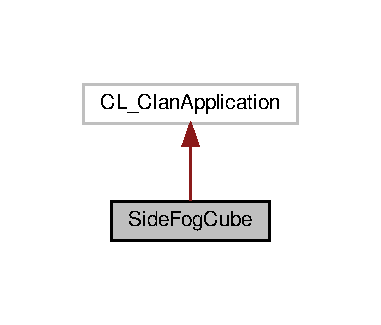
\includegraphics[width=183pt]{d4/dfd/classSideFogCube__inherit__graph}
\end{center}
\end{figure}


Collaboration diagram for Side\+Fog\+Cube\+:
\nopagebreak
\begin{figure}[H]
\begin{center}
\leavevmode
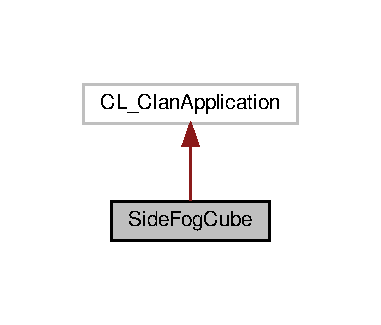
\includegraphics[width=183pt]{da/da8/classSideFogCube__coll__graph}
\end{center}
\end{figure}
\subsection*{Public Member Functions}
\begin{DoxyCompactItemize}
\item 
\hyperlink{classSideFogCube_af3f3ad8ae933d9275fb7b761c55d31fd}{Side\+Fog\+Cube} ()
\item 
virtual int \hyperlink{classSideFogCube_a54448225b0c51ba310629e606d4f512d}{main} (int argc, char $\ast$$\ast$argv)
\begin{DoxyCompactList}\small\item\em main The Clan\+Lib internal main. \end{DoxyCompactList}\end{DoxyCompactItemize}


\subsection{Detailed Description}
The class that creates a cloud of randomly spinning cubes in a fog or not. 

Definition at line 20 of file sidefogcube.\+h.



\subsection{Constructor \& Destructor Documentation}
\mbox{\Hypertarget{classSideFogCube_af3f3ad8ae933d9275fb7b761c55d31fd}\label{classSideFogCube_af3f3ad8ae933d9275fb7b761c55d31fd}} 
\index{Side\+Fog\+Cube@{Side\+Fog\+Cube}!Side\+Fog\+Cube@{Side\+Fog\+Cube}}
\index{Side\+Fog\+Cube@{Side\+Fog\+Cube}!Side\+Fog\+Cube@{Side\+Fog\+Cube}}
\subsubsection{\texorpdfstring{Side\+Fog\+Cube()}{SideFogCube()}}
{\footnotesize\ttfamily Side\+Fog\+Cube\+::\+Side\+Fog\+Cube (\begin{DoxyParamCaption}{ }\end{DoxyParamCaption})}

The cloud of cubes goes from -\/25 to 25 on all three axis. There is a light at each corner.

Definition at line 10 of file sidefogcube.\+cpp.



\subsection{Member Function Documentation}
\mbox{\Hypertarget{classSideFogCube_a54448225b0c51ba310629e606d4f512d}\label{classSideFogCube_a54448225b0c51ba310629e606d4f512d}} 
\index{Side\+Fog\+Cube@{Side\+Fog\+Cube}!main@{main}}
\index{main@{main}!Side\+Fog\+Cube@{Side\+Fog\+Cube}}
\subsubsection{\texorpdfstring{main()}{main()}}
{\footnotesize\ttfamily int Side\+Fog\+Cube\+::main (\begin{DoxyParamCaption}\item[{int}]{argc,  }\item[{char $\ast$$\ast$}]{argv }\end{DoxyParamCaption})\hspace{0.3cm}{\ttfamily [virtual]}}



main The Clan\+Lib internal main. 

Clan\+Lib uses a class internal main, nice for c++.

Create a console window for text-\/output if not available

Initialize Clan\+Lib base components

Initialize the Clan\+Lib display component

Initilize the Open\+GL drivers

Removing the true on this function will stop the program from using fullscreen.

Connect the Window close event

Connect the various signals to their slots.

Set this to true so G\+L\+EW knows to use a modern approach to retrieving function pointers and extensions

gl\+Front\+Face(\+G\+L\+\_\+\+C\+C\+W);

Define and compile the shaders.

Set the background image.

Set the foreground images.

Define the locations and image indices.

Generate the object.


\begin{DoxyEnumerate}
\item Bind the Vertex Array Object.
\item copy our vertices arrays into the buffers for Open\+GL to use. Position attribute
\end{DoxyEnumerate}

Normal attribute.

Texture attribute.

Uniform buffer to feed the uniform.

Variables for the event loop.

Initialize the random number generator.

Grab a time to count degrees by the clock.

\subsubsection*{render loop }

Grab a time to adjust camera speed.

Reset the model.

Find the camera.

render

------ Count degrees rotated.

Use the shaders.

We have a fog toggle on the space key.

Start feeding in the buffer data.

Initialize the lighting system.

Sort the locations based on the current camera position.

Set the crate background.

Set the foreground images.

Pass in the necessary uniforms.

Fog is variable based on the right arrow and left arrow keys.

Pass the image indices and cube distances.

Use the instancing feature to create multiple copies of each set of images.

Call for each image one side at a time.

Uncomment this to get a listing of the uniforms recognized by the shaders. \hyperlink{classUniformPrinter}{Uniform\+Printer} printer2(shader-\/$>$Program);

Swap buffers 



Definition at line 87 of file sidefogcube.\+cpp.



The documentation for this class was generated from the following files\+:\begin{DoxyCompactItemize}
\item 
sidefogcube.\+h\item 
sidefogcube.\+cpp\end{DoxyCompactItemize}

\hypertarget{classUniformPrinter}{}\section{Uniform\+Printer Class Reference}
\label{classUniformPrinter}\index{Uniform\+Printer@{Uniform\+Printer}}


{\ttfamily \#include $<$uniformprinter.\+h$>$}

\subsection*{Public Member Functions}
\begin{DoxyCompactItemize}
\item 
\mbox{\Hypertarget{classUniformPrinter_aae4f47e6ef97af7ee35be6df54e59ab4}\label{classUniformPrinter_aae4f47e6ef97af7ee35be6df54e59ab4}} 
\hyperlink{classUniformPrinter_aae4f47e6ef97af7ee35be6df54e59ab4}{Uniform\+Printer} (int prog\+Obj)
\begin{DoxyCompactList}\small\item\em \hyperlink{classUniformPrinter}{Uniform\+Printer} A constructor that requires the shader program object. \end{DoxyCompactList}\end{DoxyCompactItemize}
\subsection*{Protected Member Functions}
\begin{DoxyCompactItemize}
\item 
\mbox{\Hypertarget{classUniformPrinter_a54a28c69fee2cd5976b2fe725132f85d}\label{classUniformPrinter_a54a28c69fee2cd5976b2fe725132f85d}} 
void \hyperlink{classUniformPrinter_a54a28c69fee2cd5976b2fe725132f85d}{print\+Uniforms} ()
\begin{DoxyCompactList}\small\item\em print\+Uniforms Print the active uniforms. This function is little more than a giant case-\/switch statement to account for the various types of uniforms available. \end{DoxyCompactList}\end{DoxyCompactItemize}
\subsection*{Protected Attributes}
\begin{DoxyCompactItemize}
\item 
\mbox{\Hypertarget{classUniformPrinter_a36b9f4d82dd0f6cfc32cc2a3dc12790b}\label{classUniformPrinter_a36b9f4d82dd0f6cfc32cc2a3dc12790b}} 
int \hyperlink{classUniformPrinter_a36b9f4d82dd0f6cfc32cc2a3dc12790b}{max\+Uniform\+Len}
\begin{DoxyCompactList}\small\item\em Class global variables. \end{DoxyCompactList}\item 
\mbox{\Hypertarget{classUniformPrinter_a88a34ee546f9a05830c3e393b6faedf0}\label{classUniformPrinter_a88a34ee546f9a05830c3e393b6faedf0}} 
int {\bfseries num\+Uniforms}
\item 
\mbox{\Hypertarget{classUniformPrinter_a21b01430e1306d961bc654cd756f155c}\label{classUniformPrinter_a21b01430e1306d961bc654cd756f155c}} 
int {\bfseries index}
\item 
\mbox{\Hypertarget{classUniformPrinter_abc63b1870491ebccbd55684f5aa8e942}\label{classUniformPrinter_abc63b1870491ebccbd55684f5aa8e942}} 
int {\bfseries prog\+Obj}
\item 
\mbox{\Hypertarget{classUniformPrinter_a5a6265447a37c22ebf89dc15beea8818}\label{classUniformPrinter_a5a6265447a37c22ebf89dc15beea8818}} 
char $\ast$ {\bfseries uniform\+Name}
\end{DoxyCompactItemize}


\subsection{Detailed Description}
A class to encapsulate printing out the unforms from a shader program. Gives the location of the uniform and it\textquotesingle{}s status. To use this class simply instantiate it with the shader program object. 

Definition at line 22 of file uniformprinter.\+h.



The documentation for this class was generated from the following files\+:\begin{DoxyCompactItemize}
\item 
uniformprinter.\+h\item 
uniformprinter.\+cpp\end{DoxyCompactItemize}

%--- End generated contents ---

% Index
\backmatter
\newpage
\phantomsection
\clearemptydoublepage
\addcontentsline{toc}{chapter}{Index}
\printindex

\end{document}
